%%%%%%%%%%%%%%%%%%%%%%%%%BORRAR
\documentclass[a4paper]{article}
\usepackage[utf8]{inputenc}
\usepackage[spanish, es-tabla, es-noshorthands]{babel}
\usepackage[table,xcdraw]{xcolor}
\usepackage[a4paper, footnotesep = 1cm, width=18cm, left=2cm, top=2.5cm, height=25cm, textwidth=18cm, textheight=25cm]{geometry}
%\geometry{showframe}

\usepackage{tikz}
\usepackage{amsmath}
\usepackage{amsfonts}
\usepackage{amssymb}
\usepackage{float}
\usepackage{graphicx}
\usepackage{caption}
\usepackage{subcaption}
\usepackage{multicol}
\usepackage{multirow}
\setlength{\doublerulesep}{\arrayrulewidth}
\usepackage{booktabs}

\usepackage{hyperref}
\hypersetup{
    colorlinks=true,
    linkcolor=blue,
    filecolor=magenta,      
    urlcolor=blue,
    citecolor=blue,    
}
\newcommand\underrel[2]{\mathrel{\mathop{#2}\limits_{#1}}}
\newcommand{\quotes}[1]{``#1''}
\usepackage{array}
\newcolumntype{C}[1]{>{\centering\let\newline\\\arraybackslash\hspace{0pt}}m{#1}}
\usepackage[american]{circuitikz}
\usepackage{fancyhdr}
\usepackage{units} 

\graphicspath{{../Ejercicio-1/}{../Ejercicio-2/}{../Ejercicio-3/}{../Ejercicio-4/}{../Ejercicio-5/}{../Ejercicio-6/}{../Ejercicio-7/}{../Ejercicio-8/}}

\pagestyle{fancy}
\fancyhf{}
\lhead{22.13 Electrónica III}
\rhead{Mechoulam, Lambertucci, Martorell, Londero}
\rfoot{\center \thepage}
\begin{document}
\section{Aux}
\tableofcontents
%%%%%%%%%%%%%%%%%%%%%%%%%BORRAR

\subsection{Introducción}

Los mandos de control o actualmente llamados \quotes{Joysticks} son parte fundamental de varios dispositivos electrónicos utilizados hoy en día. Consolas de videojuegos, sillas de ruedas eléctricas, aeronaves radio-controladas e incluso hasta cohetes de la NASA. En su forma más básica, un potenciómetro, los mandos de control revolucionaron, al rededor de finales de la segunda guerra mundial, la manera de controlar dispositivos digitales de manera analógica. 

Esta sección del informe se centra en la implementación de un convertidor analógico a digital mediante el uso del Joystick HW-504 junto a la investigación realizada.

\subsection{Joystick HW-504}

El mando de control utilizado está compuesto por dos potenciómetros, uno para el eje X y otro para el eje Y junto a un switch accionado al apretar el mando hacia dentro. El periférico requiere de una alimentación de $5V$ y puede esquematizarse como el siguiente modelo electrónico:

\begin{figure}[H]
	\begin{subfigure}[t]{0.49\textwidth}
		\centering
		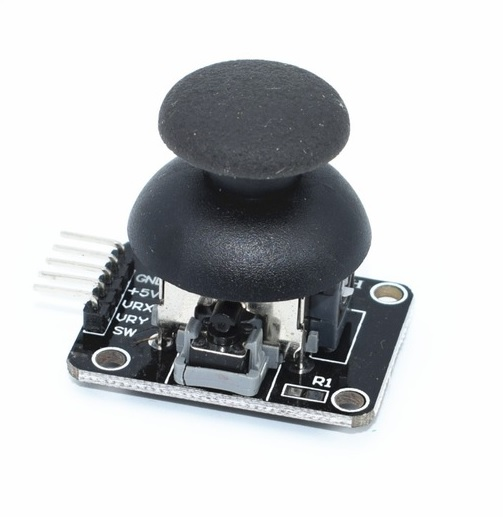
\includegraphics[width=0.6\textwidth]{Imagenes/joystick.jpg}
		\caption{Mando de control HW-504 utilizado.}
		\label{fig:joystick}
	\end{subfigure}
	\begin{subfigure}[t]{0.49\textwidth}
		\centering
		\scalebox{0.7}{
		\begin{circuitikz}

		\draw

		(-3,0) node[label=west:{\color{blue}\textbf{+5V}}](5V){}
			to[short,o-*] ++ (2, 0)
			node[](LEFT_POTX_NODE){}
	
		(LEFT_POTX_NODE) to[pR, -*, name=pot-x] ++ (5, 0)
			node[](RIGHT_POTX_NODE){}

		(pot-x.wiper) to[short, -o] ++ (0, 0)
			node[label=north:{\color{blue}\textbf{VRx}}](){}

		(LEFT_POTX_NODE) to[short] ++ (0, -1.6)
			node[](LEFT_POTY_NODE){}
			to[pR, name=pot-y] ++ (5, 0)
			node[](RIGHT_POTY_NODE){}
	
		(pot-y.wiper) to[short, -o] ++ (0,0)
			node[label=north:{\color{blue}\textbf{VRy}}](){}
	
		%(LEFT_POTY_NODE) to[short] ++ (0, -1.7)
			%node[](LEFT_SW_NODE){}
			%to[push button] ++ (5, 0)
			%to[short, -o] ++ (2,0)
			%node[label=east:{\color{blue}\textbf{SW}}](SW){}
	
		(RIGHT_POTX_NODE) to[short] ++ (0, -1.6)

		(RIGHT_POTX_NODE) to[short, -o] ++ (2, 0)
	
			node[label=east:{\color{blue}\textbf{GND}}](GND){}
			
		to[open] ++ (0, -5.5)

		(GND) ++ (-1.5, 0) to[open] ++ (0, -2.55)
			to[open] ++ (-5.5, 0)
			to[open] ++ (0, -0.8)
			to[open] ++ (1.5,0)
			node[](a1){}
			to[push button] ++ (2, 0)
			node[](a2){}
		(RIGHT_POTY_NODE) to [short] ++ (0,-1.75)
			to[short] (a2)
		(a1) to[short,-o] ++ (-3.5,0)
		node[label=west:{\color{blue}\textbf{SW}}](SW){}
		
		;

		\end{circuitikz}
		}
		\caption{Circuito equivalente del mando HW-504 con mismos nombres que el pin-out del periférico.}
		\label{circuit:joytick_eq}
	\end{subfigure}
\end{figure}

Como se puede observar en la Figura (\ref{circuit:joytick_eq}), la tensión en los pines $VR_x$ y $VR_y$ será proporcional a la posición del joystick, mientras que el pin $SW$ permanecerá en estado alto a menos que se presione el mando. Los potenciómetros del joystick son ambos de $10k\Omega$.

\subsection{Diseño Propuesto}

\subsubsection{Breve Descripción}

\begin{figure}[H]
	\centering
	\scalebox{0.9}{
	\centering
	\begin{circuitikz}
		\draw	
	
			node[fourport](CLK){}
			node[]{CLK Gen}
			
			to[open] ++ (-3, 0) node[fourport, xscale=1.5, yscale=0.7](INPUTDRIVER){}
			node[]{Input Driver}
			
			(CLK) ++ (3, 1.5) node[fourport](CLK/100){}
			node[]{\LARGE{$\frac{f}{100}$}}
			
			++ (3, 0) node[fourport](INTEGRATOR){}
			node[]{\LARGE{$\int$ + G}}

			++ (3.5, 0) node[fourport, xscale=1.5](COMPARATOR){}
			node[]{\large{Comparator}}
			
			++ (3.5, 0) node[fourport](JOYSTICK){}
			node[]{\large{Joystick}}
						
			(CLK) ++ (3.5, -1.5) node[fourport, xscale=1.5](COUNTER){}
			node[]{\large{Counter 0-99}}
			
			(COMPARATOR) ++ (0, -1.5) node[fourport, xscale=1.5, yscale=0.3](EDGEDETECTOR){}
			node[]{Edge Detector}
			
			(EDGEDETECTOR) ++ (0, -1.5) node[fourport](DISPLAY){}
			node[]{Display}
			
			(CLK/100) to[open] ++ (0.5, -1.5) node[fourport, xscale=1.5, yscale=0.3](EDGEDETECTOR2){}
			node[]{Edge Detector}
			
			(CLK.east) to[short] ++ (0.5, 0)
				|- (CLK/100.west)
				
			(CLK.east) to[open] ++ (0.5,0)
				|- (COUNTER.west)
			
			(CLK/100.east) -- (INTEGRATOR.west) 
			(INTEGRATOR.east) -- (COMPARATOR.west)
			(COMPARATOR.east) -- (JOYSTICK.west)
			(COMPARATOR.south) -- (EDGEDETECTOR.north)
			(EDGEDETECTOR.south) -- (DISPLAY.north)
			(COUNTER.east) -- (DISPLAY.west)
			(EDGEDETECTOR2.north) ++ (-0.5, 0) -- (CLK/100.south)
			(EDGEDETECTOR2.south) -- (COUNTER.north) 
			(CLK.west) -- (INPUTDRIVER.east)
		;
	\end{circuitikz}
	}
	\caption{Diagrama en bloques del diseño propuesto.}
	\label{circuit:dis}
\end{figure}

Se propuso el diseño presentado en la Figura (\ref{circuit:dis}). Este consta de un generador de clock que varía entre $100Hz$ y $2KHz$ el cual es provisto a un contador BCD el cual se reinicia al llegar al numero 99. Este contador posee sus salidas conectadas permanentemente a un módulo de display el cual tiene una entrada de acquire, la cual al pasar a estar en un estado alto el display muestra y guarda el último número ingresado aun así este pin pase a un estado bajo.

Por otro lado, el generador de clock está también conectado a otro módulo, el cual divide la frecuencia del clock por cien, resultando en un segundo clock sincronizado con el primero de una frecuencia variable entre $1Hz$ y $20Hz$. Esta señal cuadrada de frecuencia cien veces menor a la original, es ingresada a un integrador. Este último, genera a partir de dicha señal, una rampa la cual atraviesa posteriormente una etapa de amplificación. El valor de tensión de la rampa es permanentemente comparado con el valor de tensión del pin de posición del joystick, de tal manera que, apenas sea la tensión de la rampa mayor a la tensión provista por el joystick, el comparador pondrá su salida en un estado alto. Esta salida está conectada a un detector de flancos, y es este flanco el que ingresa al pin de acquire del display, obteniendo en este siempre la posición del joystick mapeada de 0 a 99.

Por último, la señal del contador de frecuencia dividida por cien, la cual se utiliza para la generación de la rampa, es ingresada también a otro detector de flancos el cual ingresa al pin de reset del contador BCD. Esto genera que siempre que comience la rampa el contador sea reseteado a 00.

\subsubsection{Input Driver}

Se buscó realizar un diseño autónomo que funcione con dos baterías de $9V$. Para esto, se utilizó una etapa de entrada compuesta por el regulador de tensión \href{https://www.sparkfun.com/datasheets/Components/LM7805.pdf}{LM7805}. Esta etapa de entrada proporcionará los $5V$ que alimentarán todos los integrados digitales del diseño.

\subsubsection{Clock Generator}

Para el generador de clock se utilizó el famoso integrado \href{http://www.ti.com/lit/ds/symlink/se555.pdf}{NE555}. Este integrado está compuesto por dos comparadores (cuyo funcionamiento se encuentra detallado más adelante), un SR-Latch, un transistor de descarga y finalmente un driver de salida, como se observa en la Figura (\ref{fig:555}).

\begin{figure}[H]
	\centering
	\scalebox{0.7}{
	\begin{circuitikz}
		\draw	
		
		%%%%%%%%%%%%%%%%%%%%%%%%%%%%%%%%%%%%%%%%%%%%%%%%%%%%%%%%%%%%
		%Setting figures
		%%%%%%%%%%%%%%%%%%%%%%%%%%%%%%%%%%%%%%%%%%%%%%%%%%%%%%%%%%%%
		node[op amp](op1){} %Opamp1
			to[open] ++ (-0.1, -0.3)
			node[label=\tiny{Comparator}]{}
			to[open] ++ (0,0.2)
		to[open] ++ (0, -3)
		
		node[op amp, yscale=-1](op2){} %Opamp2
			to[open] ++ (-0.1, -0.3)
			node[label=\tiny{Comparator}]{}
			to[open] ++ (0,0.2)
		to[open] ++ (3, 1.5)
		
		node[fourport](srlatch){} %SR-Latch
			(srlatch.1) ++ (0.3, -0.3) node[label=$S$]{}
			(srlatch.2) ++ (-0.3, -0.3) node[label=$\overline{Q}$]{}
			(srlatch.3) ++ (-0.3, -0.3) node[label=$Q$]{}
			(srlatch.4) ++ (0.3, -0.3) node[label=$R$]{}
		to[open] ++ (4, 2)
		
		node[npn](npn){} %Neperiano
			(npn.E) node[tlground]{}

		(srlatch.2) ++ (2.5, 0) node[fourport, label=center:OUT, scale = 0.5](outdriver){}
		%%%%%%%%%%%%%%%%%%%%%%%%%%%%%%%%%%%%%%%%%%%%%%%%%%%%%%%%%%%%
		%NODES:
		%	op1, op2, srlatch, npn, outdriver
		%
		%%%%%%%%%%%%%%%%%%%%%%%%%%%%%%%%%%%%%%%%%%%%%%%%%%%%%%%%%%%%
		(op1.out) |- (srlatch.4)
		
		(op2.out) |- (srlatch.1)
		
		(srlatch.3) to[short] ++ (0.5, 0)
			node[plain crossing, rotate=45]{}
		
		(srlatch.2) to[short, o-o] (outdriver.west)
			to[open, -*] ++ (-1, 0)
			|- (npn.B)
			
		(npn.C) to[short, -o] ++ (0, 1.75)
			node[label=north:DISCHARGE]{}
			node[label=west:7]{}
			
		(outdriver.east) to[short, -o] ++ (2, 0)
			node[label=east:OUT]{}
			node[label=north:3]{}
			
		(srlatch.north) to[short, o-o] ++ (0, 3.75)
			node[label=north:RESET]{}
			node[label=west:4]{}
		
		(op1.-) to[short, -*] ++ (-0.5, 0)
			to[short] ++ (0, 2.5)
			node[ocirc, label=north:CONTROL VOLT]{}
			node[label=west:5]{}		
			to[open] ++ (0, -2.5)
			to[short, -*] ++ (-2.5, 0)
			to[R, l_=$5K$, -o] ++ (0, 2.42)
			node[label=north:VCC]{}
			node[label=west:8]{}
			to[open] ++ (0, -2.42)
			to[R, l=$5K$, -*] ++ (0, -3.1)
			node(aux){}
			to[R, l=$5K$, -o] ++ (0, -3)
			node[label=south:GND]{}
			node[label=west:1]{}


		(op1.+) to[short] ++ (-1.2, 0)
			to[short] ++ (0, 0.5)
			to[short, -o] ++ (-3, 0)
			node[label=north:6]{}
			node[label=west:THRESHOLD]{}

		(op2.+) to[short] ++ (-2.94, 0)
		
		(op2.-) to[short] ++ (-1.2, 0)
			to[short] ++ (0,0.5)
			to[short, -o] ++ (-3, 0)
			node[label=north:2]{}
			node[label=west:TRIGGER]{}
		
		;
	\end{circuitikz}
	}
	\caption{Diagrama en bloques del integrado 555.}
	\label{fig:555}
\end{figure}

Colocando un capacitor a tierra conectado al pin de trigger y threshold, se puede utilizar la carga y descarga de este para ser comparado con un nivel de tensión de referencia, generalmente $\frac{2}{3} V_{CC}$. Cuando la tensión del capacitor excede este valor, se activa el transistor de descarga del integrado, descargando rápidamente al capacitor y generando que el comparador ponga en un estado bajo a la salida del integrado. Esto provoca una señal cuadrada cuyo duty-cycle y frecuencia puede ser modificada mediante resistencias o potenciómetros que causan una carga y descarga más lenta del capacitor. 

Las ecuaciones que controlan la frecuencia y duty-cycle del generador son detalladas a continuación. Cabe notar que el capacitor C y las resistencias $R_1$ y $R_2$ no se encuentran dibujadas en la Figura (\ref{fig:555}).

\begin{equation}
t_{on} = 0.639\cdot C \cdot R_1
\end{equation}
\begin{equation}
t_{off} = 0.639 \cdot C \cdot (R_1 + R_2)
\end{equation}
\begin{equation}
f=\frac{1}{t_{off} + t_{on}}
\end{equation}

Se colocó un potenciómetro en la resistencia $R_2$ de tal manera que cuando este se encuentre en $0\%$ la frecuencia de la señal de salida sea de $2KHz$ mientras que si el potenciómetro se encuentra en su máxima resistencia la frecuencia de la señal de salida sea de $100Hz$. Cabe notar que cuando la frecuencia del generador de clock decrece, lo que sucede es que solamente aumenta el periodo de tiempo en el que la salida se encuentra en un estado bajo.

\subsubsection{Frequency Divider}

Para el divisor de frecuencia se utilizaron los dos contadores en década del integrado \href{http://www.ti.com/lit/ds/symlink/cd4017b.pdf}{CD4017BE}. Conectando el pin de carry out, el cual se enciende una vez cada diez señales de clock, a la entrada de clock del segundo contador se logra obtener a la salida del segundo contador una señal de clock cuya frecuencia es cien veces menor a la original. Una buena característica de este diseño es que no solo el clock original esta completamente sincronizado con esta nueva señal de clock cien veces más lenta, sino que por la naturaleza del funcionamiento interno de estos contadores, el duty-cycle de este nuevo clock es siempre del $50\%$. Esto prueba ser muy beneficioso a la hora de integrar esta señal para conseguir una rampa.

\subsubsection{Integrador}

Para la etapa de generación de rampa se decidió construir un integrador compensado con un amplificador operacional seguido de una etapa de amplificación compuesta por otro operacional en configuración inversora, ya que el integrador invierte la señal que este integra. Como la señal integrada es el segundo clock generado, y este está en sincronía con el primero, se puede efectivamente utilizar el clock original para contar cien pulsos dentro de la duración de la rampa. Los dos operacionales utilizados son los del integrado \href{http://www.ti.com/lit/ds/symlink/tl082.pdf}{TL-082}.

\subsubsection{Comparador}

Se utilizó el integrado \href{http://www.ti.com/lit/ds/symlink/lm211.pdf}{LM311} para comparar la tensión proveniente del joystick con la tensión de la rampa. El comparador más genérico puede ser construido con un solo amplificador operacional a lazo abierto como se observa en la Figura (\ref{circ:comparador}).

\begin{figure}[H]

	\centering
	\begin{circuitikz}
		\draw	
	
			node[op amp](opamp){}
			
			(opamp.up) to[short, -*] ++ (0, 2)
				to[open] ++ (-4, 0)
				node[label=west:$V_{CC}$]{}
				to[short, o-] ++ (8, 0)
			
			(opamp.down) to[short, -*] ++ (0, -2)
				to[open] ++ (-4, 0)
				node[label=west:$GND$]{}
				to[short, o-] ++ (8, 0)
				
			(opamp.-) to[short] ++ (-0.5, 0)
				node[label=west:$V_{REF}$]{}				
				to[R, l=$R_1$, *-*] ++ (0, 2)
				to[open] ++ (0, -2)
				to[short] ++ (0, -1)
				to[R, l=$R_2$, -*] ++ (0, -2.03)			
			
			(opamp.+) to[short] ++ (-1, 0)
				to[short, -o] ++ (-2, 0)
				node[label=west:$V_{in}$]{}
	
			(opamp.out) to[short, -o] ++ (2.75, 0)
				node[label=east:$V_{out}$]{}
	
		;
	\end{circuitikz}
	\caption{Amplificador operacional en configuración comparador.}
	\label{circ:comparador}
\end{figure}

Las ecuaciones que gobiernan la salida de este son:

\begin{equation*}
V_{out} = A_0 (V_{in} - V_{REF}) \approx
\left\{
\begin{aligned}
		& V_{CC} \ \ \ \ \ si \ \ V_{in} > V_{REF} \\		
		& 0 \ \ \ \ \ \ \ \ \ si \ \ V_{in} < V_{REF}\\		
\end{aligned}
\right.
\end{equation*}


\subsubsection{Counter}

Se utilizaron por comodidad contadores BCD en cascada, conectando al enable del segundo contador los pines ``1'' y ``8'' del primero, lo que efectivamente genera que el segundo contador solamente se incremente cuando el primero tenga un valor igual a 9. Se utilizaron los integrados \href{http://www.ti.com/lit/ds/symlink/cd4518b.pdf}{CD4518BE}.

Para sincronizar estos contadores se utilizó el flanco ascendente del clock lento el cual marca el comienzo de la rampa. Este flanco es ingresado al pin de reset de ambos contadores primero siendo invertido ya que estos contadores poseen pin de reset activo bajo.

\subsubsection{Edge Detector}

Para los detectores de flancos se decidió utilizar particularmente un diseño entre varios propuestos. Este se detalla en la Figura (\ref{circ:edge}).

\begin{figure}[H]
	\centering	
\begin{circuitikz}
	\draw
		node[fourport](FF){}
			(FF.east) ++ (0, 0.5) to[short] ++ (1, 0)
			to[open] ++ (0.7,0)
			node[not port](not){}
			to[open] ++ (0.7, 0)
			to[short] ++ (1, 0)
			to[open] ++ (1.39, 0.28)
			node[and port](and){}
			(FF.east) ++ (-0.25,0.5)
			node[](Q){$Q$}
			(FF.east) ++ (-0.25, -0.5)
			node[](-Q){$\overline{Q}$}
			(FF.west) ++ (0.25, 0.5)
			node[](D){$D$}
			(FF.west) ++ (0.1,-0.5)
			node[](CLK){\scalebox{1.2}{\rotatebox{-90}{$\triangle$}}}
		(and.in 1) to[short] ++ (0, 0.5)
			to[short] ++ (-6, 0)
			to[short, -*] ++ (0, -1.05)
		(D) ++ (-0.25, 0) to[short, -o] ++ (-2, 0)
			node[label=west:$PULSE$]{}
		
		(and.out) to[short, -o] ++ (0.75, 0)
		node[label=east:$EDGE$] {}
		(CLK) ++ (-0.25, 0) to [short, -o] ++ (-2, 0)
		node[label=west:$CLK$] {}
	;
\end{circuitikz}
\caption{Detector de flancos utilizado.}
\label{circ:edge}
\end{figure}

El funcionamiento de este se basa en que el flanco a la salida tendrá siempre una duración menor a la del clock utilizado. Esencialmente, cuando la entrada se mantiene en bajo, el flip-flop tendrá guardado un estado bajo, por lo que al terminal de la compuerta AND le llegará un uno, mientras que a la otra terminal de la AND le llegara un cero. Cuando la señal de entrada pase a alto, la salida será alta hasta el próximo clock el cual pondrá la salida del flip-flop en bajo, poniendo un cero a la salida EDGE. El integrado utilizado fue el \href{http://www.ti.com/lit/ds/symlink/cd4013b.pdf}{CD4013BE}.


\subsubsection{Display}

Se utilizaron decoders de BCD a 7 segmentos para realizar el módulo del display. La salida de los contadores es permanentemente ingresada a estos decodificadores. Sin embargo, los decoders poseen un pin que debe estar en bajo para refrescar su salida. Si este pin se encuentra en un estado alto, el decodificador no actualiza su salida, sino que mantiene a esta en el último estado en el que estuvo. Es a este pin al cual le ingresa la señal de acquire, que es la salida del comparador la cual es ingresada a un detector de flancos. Esto genera que el valor que es mostrado en los displays sea el de los contadores solamente cuando la tensión de la rampa sea igual a la del joystick. Cuando esto no se cumple, el display muestra el ultimo valor mostrado.
El decoder utilizado fue el \href{http://www.ti.com/lit/ds/schs279d/schs279d.pdf}{CD74HC4511E}. Mientras que los displays utilizados fueron los de configuración cátodo común, ya que la corriente proporcionada por los 4511 era la suficiente para encender todos los segmentos.

\subsection{Simulaciones}
Se simuló a cada módulo por separado. Para esto, se utilizó el software \textit{LTSpice XVII} para lo analógico y \textit{Proteus 8} para lo digital. 
El generador de rampa si bien no es totalmente lineal, asumimos la imprecisión que esto generaría como despreciable para nuestra aplicación.
\begin{figure}[H]
\centering
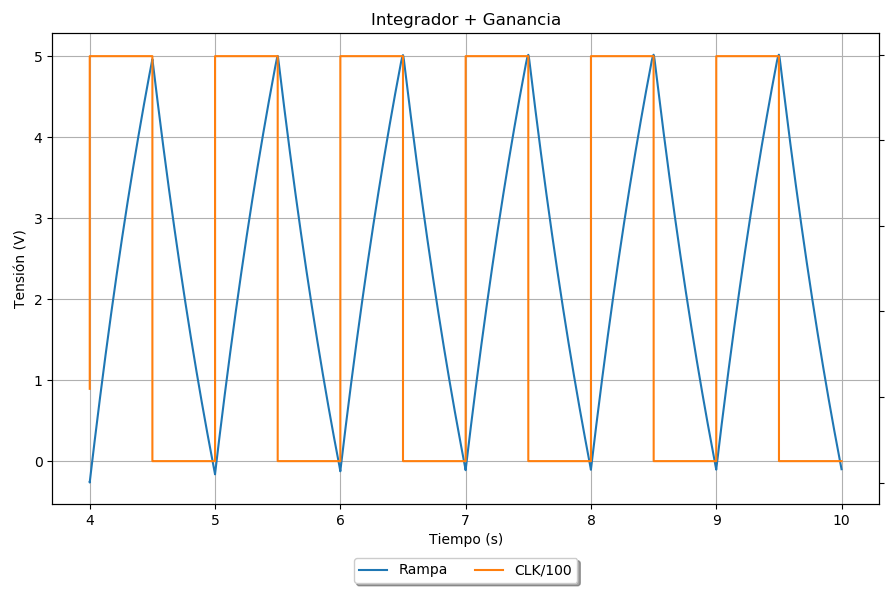
\includegraphics[width=0.8\textwidth]{Imagenes/sqare.png}
\caption{Simulación del generador de rampa.}
\label{sim:ramp}
\end{figure}
Luego, el divisor de frecuencia simulado en Proteus demuestra un correcto funcionamiento. Dado un clock de $100Hz$, se logra obtener otro de $1Hz$.
\begin{figure}[H]
\centering
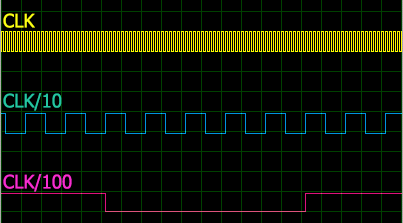
\includegraphics[width=0.8\textwidth]{Imagenes/freqdiv.png}
\caption{Simulación del divisor de frecuencia.}
\label{sim:freqdiv}
\end{figure}
Para el generador de clocks se simuló con el preset tanto en su mínima resistencia como en su máxima resistencia. Se logró obtener en estas dos configuraciones una frecuencia ajustable entre $91.44Hz$ y $1993Hz$.
\begin{figure}[H]
\centering
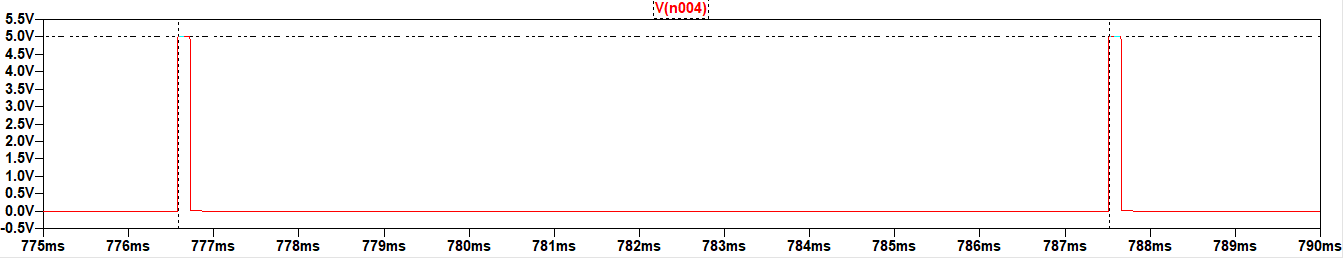
\includegraphics[width=\textwidth]{Imagenes/clockgen1.png}
\caption{Simulación del generador de clock con una frecuencia de $91.44Hz$.}
\label{sim:gen1}
\end{figure}
\begin{figure}[H]
\centering
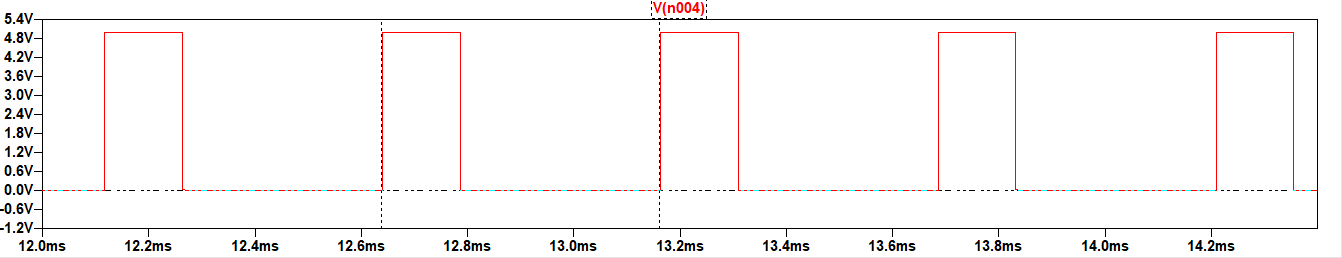
\includegraphics[width=\textwidth]{Imagenes/clockgen2.png}
\caption{Simulación del generador de clock con una frecuencia de $1993.4Hz$.}
\label{sim:gen2}
\end{figure}

No se realizaron simulaciones para el comparador, el contador o el regulador de tensión ya que están constituidos por solamente el integrado que realiza su función.

\subsection{Implementación y Mediciones}
Se implementó el circuito en un PCB de 10x20. A la placa se le añadieron jumpers para desconectar el generador de rampa del resto para así poder calibrarlo. Se midió este ingresando un clock generado por un generador de funciones obteniendo la siguiente respuesta.

\begin{figure}[H]
\centering
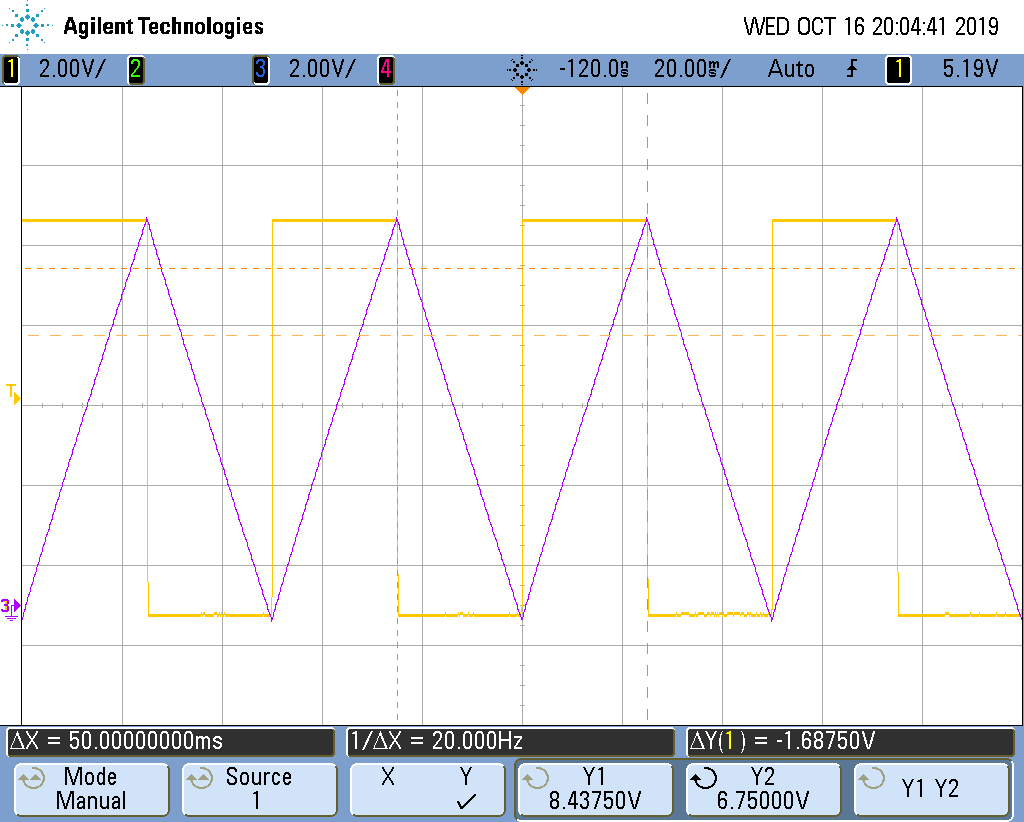
\includegraphics[width=\textwidth,trim={0 2.2cm 0.1cm 1.75cm},clip]{Imagenes/ramp.png}
\caption{Medición y calibración del generador de rampa con un clock provisto por un generador de funciones.}
\label{med:ramp}
\end{figure}

Luego, se comprobó el correcto funcionamiento del diseño en su totalidad.
\end{document}